%\documentclass[14pt]{beamer}
\documentclass{beamer}

\usetheme{Copenhagen}
% \usetheme{Boadilla}
% \usecolortheme{beaver}
\setbeamercolor{alerted text}{fg=orange}
\setbeamercolor{background canvas}{bg=white}
\setbeamercolor{block body alerted}{bg=normal text.bg!90!black}
\setbeamercolor{block body}{bg=normal text.bg!90!black}
\setbeamercolor{block body example}{bg=normal text.bg!90!black}
\setbeamercolor{block title alerted}{use={normal text,alerted text},fg=alerted text.fg!75!normal text.fg,bg=normal text.bg!75!black}
\setbeamercolor{block title}{bg=blue}
\setbeamercolor{block title example}{use={normal text,example text},fg=example text.fg!75!normal text.fg,bg=normal text.bg!75!black}
\setbeamercolor{fine separation line}{}
\setbeamercolor{frametitle}{fg=white}
\setbeamercolor{item projected}{fg=white}
\setbeamercolor{normal text}{bg=white,fg=black}
\setbeamercolor{palette sidebar primary}{use=normal text,fg=normal text.fg}
\setbeamercolor{palette sidebar quaternary}{use=structure,fg=structure.fg}
\setbeamercolor{palette sidebar secondary}{use=structure,fg=structure.fg}
\setbeamercolor{palette sidebar tertiary}{use=normal text,fg=normal text.fg}
\setbeamercolor{section in sidebar}{fg=brown}
\setbeamercolor{section in sidebar shaded}{fg=grey}
\setbeamercolor{separation line}{}
\setbeamercolor{sidebar}{bg=red}
\setbeamercolor{sidebar}{parent=palette primary}
\setbeamercolor{structure}{bg=black, fg=white!30!blue!60!green}
\setbeamercolor{subsection in sidebar}{fg=brown}
\setbeamercolor{subsection in sidebar shaded}{fg=grey}
\setbeamercolor{title}{fg=white}
\setbeamercolor{titlelike}{fg=white}

% Szép kék
% \setbeamercolor{structure}{bg=black, fg=white!10!green!40!blue}

\frenchspacing

% Language packages
\usepackage[utf8]{inputenc}
\usepackage[T1]{fontenc}
\usepackage[magyar]{babel}

% AMS
\usepackage{amssymb,amsmath}

% Graphic packages
\usepackage{graphicx}

% Syntax highlighting
\usepackage{listings}

\usepackage{tikz}

%\begin{figure}[htb]
%\begin{center}
%	\includegraphics[scale=0.4]{ps_times.png}
%\end{center}
%\end{figure}

\usefonttheme{professionalfonts} % using non standard fonts for beamer
\usefonttheme{serif} % default family is serif
\usepackage{tgbonum}

% ==============
\begin{document}
% ==============

\title[Strukturált adatok kinyerése PDF dokumentumokból]{Strukturált adatok kinyerése PDF dokumentumokból}
\author[Molnár Fanni]{\textbf{Molnár Fanni}}
\institute[]{Miskolci Egyetem}
\date{2020. június 23.}

% --------------------
\frame{\titlepage}

% --------------------
\begin{frame}[fragile]
\frametitle{Bevezetés}

A dokumentumaink egy jelentős része elektronikus formában érhető el. Ennek közkedvelt formátuma a PDF (Portable Document Format).
A dolgozat olyan módszereket mutat be, amelyek a képek strukturális elemeit ismerik fel.

\smallskip

Az elemzésnek két fő alternatívája lehet:

\bigskip

\begin{itemize}
    \item PDF API-k használatával lehet kinyerni a fájlokból a dokumentum adatait
    \item PDF képpé alakítása, majd képfeldolgozási módszerekkel való elemzése
\end{itemize}

\end{frame}

% --------------------
\begin{frame}[fragile]
\frametitle{Dokumentum szerkezete}

A dokumentumok szerkezete lehet nagyon egyszerű, de igen komplikált is.

\smallskip

\begin{figure}[!tbp]
  \centering
  \begin{minipage}[b]{0.45\textwidth}
    
\includegraphics[width=\textwidth]{images/page_simple.png}
  \end{minipage}
  \hfill
  \begin{minipage}[b]{0.45\textwidth}
    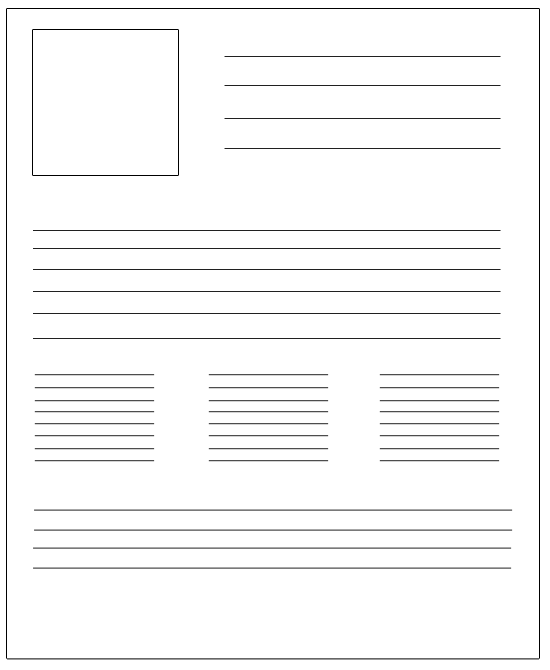
\includegraphics[width=\textwidth]{images/page_complicated.png}
  \end{minipage}
\end{figure}

\end{frame}

% --------------------
\begin{frame}[fragile]
\frametitle{Dokumentum felbontása}

A felbontásokhoz a dokumentumban levő, összefüggő fehér területeket kerestem (margó, sorköz stb.). Meghatároztam az intenzitást a dokumentum minden sorára és oszlopára majd ezek mentén kezdtem meg a felbontást.

\smallskip

\begin{figure}[!tbp]
  \centering
  \begin{minipage}[b]{0.45\textwidth}
    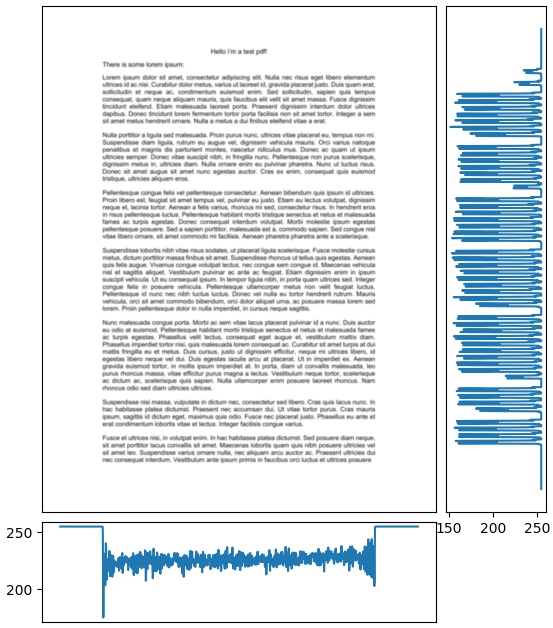
\includegraphics[width=\textwidth]{images/intensity.png}
  \end{minipage}
\end{figure}

\end{frame}

% --------------------
\begin{frame}[fragile]
\frametitle{Margók}

A margók levágásához az intenzitásokat tartalmazó tömb elejétől indultam el, majd addig haladtam amíg fehér, egybefüggő területet találtam. Amint az intenzitás nem 255, abban az esetben megállok, és lementem az indexet, mivel onnantól kezdődik a dokumentum első szöveget tartalmazó sora. Ezt megismétlem visszafelé is mind a kettő tömbön, így lesz meg alsó-felső, jobb-bal margó végpontja.

\bigskip

A kapott margók nélküli dokumentumot fogom tovább bontani paragrafusokra, sorokra, szavakra majd karakterekre.

\end{frame}

% --------------------
\begin{frame}[fragile]
\frametitle{Paragrafusok}

A paragrafusokra bontásnál azt feltételezem hogy a térköz nagyobb mint a sorköz.
\newline
Eleinte csak egy tapasztalati értéket használtam (40 feletti közök), de a későbbiekben készítettem egy küszöbérték becslést, ahol a vizsgálat elején meghatároztam a margókat, térközt, sorközt és később azokkal az értékekkel dolgoztam.

\bigskip

A tapasztalti értékemet a lent látható hisztogramra alapoztam.

\begin{figure}[!tbp]
  \centering
  \begin{minipage}[b]{0.45\textwidth}
    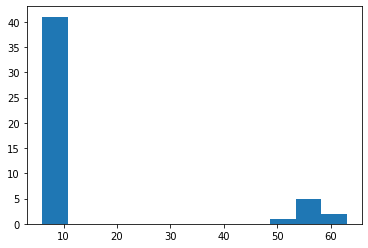
\includegraphics[width=\textwidth]{images/segment_hist.png}
  \end{minipage}
\end{figure}

\end{frame}

% --------------------
\begin{frame}[fragile]
\frametitle{Sorok}

A soroknál ugyan azon algoritmussal dolgoztam mint a paragrafusoknál, annyi különbséggel hogy itt a küszöbérték az sokkal alacsonyabb volt.

\bigskip

Kezdetben itt is tapasztalati küszöbértéket használtam, méghozzá a 4-től nagyobb összefüggő területeket kerestem. Úgy tapasztaltam hogy alatta a sötét részek főleg zajok, nem pedig teljes sorok.

\end{frame}

% --------------------
\begin{frame}[fragile]
\frametitle{Szavak}

A szavakra és karakterekre bontást már nem az y, hanem az x tengely mentén végeztem.

\bigskip

A már kivágott sorokat felhasználva kerestem a fehér területeket, tapasztalati érték alapján legalább 5 darabot, majd egyenként lementettem a megtalált szavakat.

\end{frame}

% --------------------
\begin{frame}[fragile]
\frametitle{Karakterek}

A szavak betűkre bontása már egy érdekesebb témakör. Ennél az algoritmusnál már nem a világos, hanem épp hogy a sötét részeket kerestem, és ha már 1 pixelnek megfelelő sötét részt is találtam már mentettem az adott indexet.

\bigskip

Ez a legtöbb esetben szépen működött, és megkaptam egyesével a betűket.

\bigskip

Viszont a ligatúrák esetében a karakterek egymásba lógnak, ezért az algoritmusom nem vágta szét őket, hanem egybe mentette le.
Ilyen esetek voltak például az r és az f vagy t találkozása, vagy például a dupla t vagy f betűk.

\begin{figure}[!tbp]
  \centering
  \begin{minipage}[b]{0.45\textwidth}
    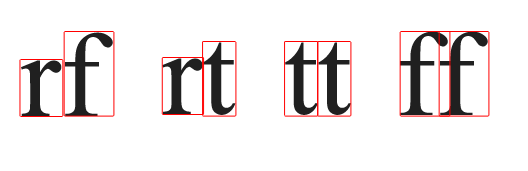
\includegraphics[width=\textwidth]{images/ligatura.png}
  \end{minipage}
\end{figure}

\end{frame}

% --------------------
\begin{frame}[fragile]
\frametitle{Bonyolultabb dokumentum felbontása}

Bonyolultabb dokumentumok esetében nem elég az y tengely menti vizsgálat, hanem minden kivágott bekezdés esetén meg kell vizsgálni, hogy az adott bekezdés tartalmaz-e több paragrafust.
Ha igen, azokat is külön kell választanunk.

\begin{figure}[!tbp]
  \centering
  \begin{minipage}[b]{0.3\textwidth}
    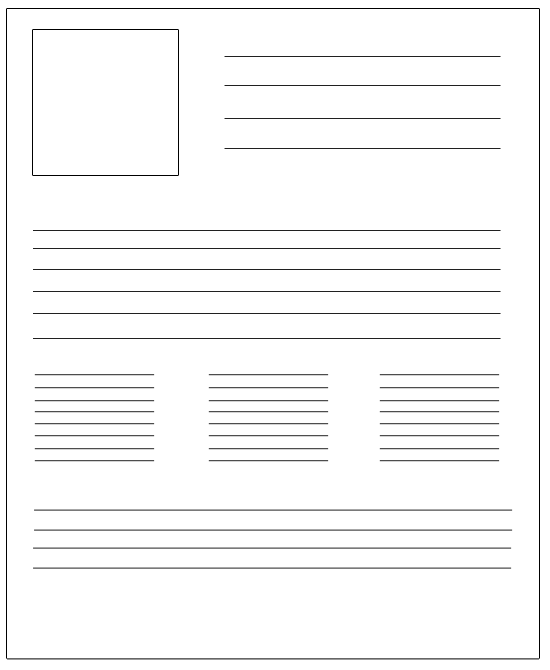
\includegraphics[width=\textwidth]{images/page_complicated.png}
  \end{minipage}
  \hfill
  \begin{minipage}[b]{0.3\textwidth}
    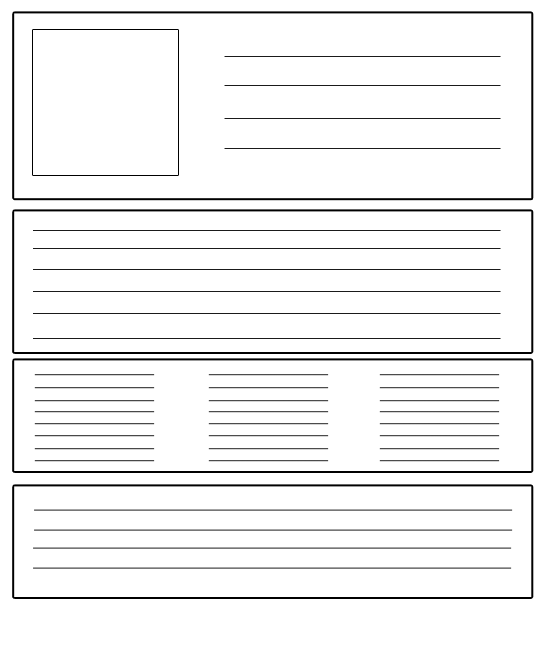
\includegraphics[width=\textwidth]{images/page_complicated2.png}
  \end{minipage}
  \hfill
  \begin{minipage}[b]{0.3\textwidth}
    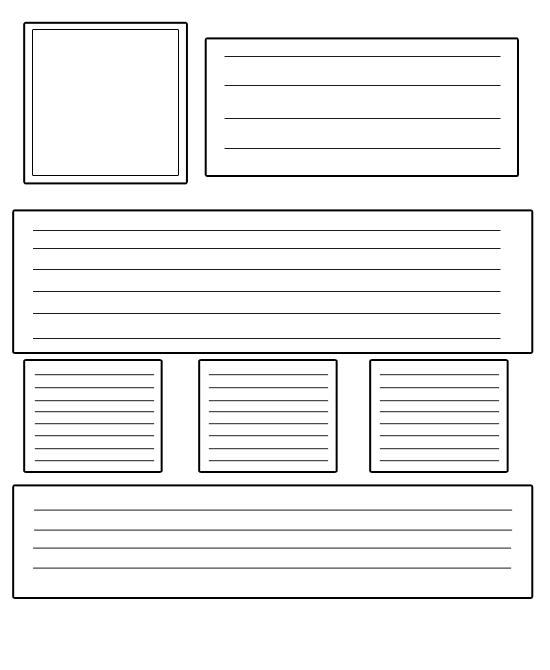
\includegraphics[width=\textwidth]{images/page_complicated3.png}
  \end{minipage}
\end{figure}

\end{frame}

% --------------------
\begin{frame}[fragile]
\frametitle{Képek és szövegek megkülönböztetése}

 Ha tartalmaz képet a dokumentumunk, azt meg kell különböztetnünk a bekezdésektől. Ehhez kezdetben azt a tényt használtam fel hogy a szöveget tartalmazó képnél kell legyen összefüggő világos intenzitás (háttér), majd egy sötétebb intenzitás (ami a szöveg) majd még egy egybefüggő világos intenzitás. Sajnos ez a módszer nem volt túl hatékony.

\begin{figure}[!tbp]
  \centering
  \begin{minipage}[b]{0.45\textwidth}
    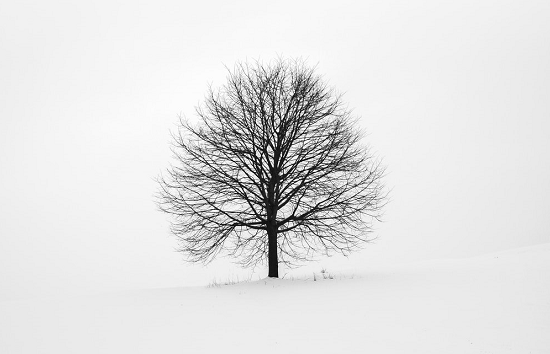
\includegraphics[width=\textwidth]{images/tree.png}
  \end{minipage}
\end{figure}

\end{frame}

% --------------------
\begin{frame}[fragile]
\frametitle{Képfelismerés neurális háló segítségével}

A képfelismerés javításának érdekében a Python-ban megtalálható Keras nevezetű neurális háló API-val kezdtem el foglalkozni.
A Keras fő építőeleme a modell, ami lehetőséget ad a különböző rétegek kezelésére.
Első lépésben konfigurálni kell a modellünket, megadni hogy hány és milyen rétegeket szeretnénk használni, majd következik a betanítás.

\bigskip

Egy szekvenciális modellt használtam, 2 konvolúciós és 2 pooling réteggel. A betanítás során 150 képet adtam be a modellemnek, egyenként 32 × 32-es méretűeket.
Ahhoz, hogy pontosabb eredményt érjünk el, sokkal több tanuló képre lenne szükség de a programomban a kép és szöveg megkülönböztetése nagyban javult, így ezzel elértem a célomat.

\end{frame}

% --------------------
\begin{frame}[fragile]
\frametitle{Összegzés}

\begin{itemize}
    \item A szerkezeti elemzés bizonyos dokumentumok esetében nagyon bonyolult
    \item A felvetett problémára csak akkor lehetne tökéletes megoldást adni, hogy ha pontosan definiálva lenne, hogy milyen elemek és hogyan fordulhatnak elő egy dokumentumban
\end{itemize}

\end{frame}

% --------------------
\begin{frame}[fragile]
\frametitle{\ }

\begin{center}

    \Large

    \textbf{Köszönöm szépen a figyelmet!}

    \bigskip

\end{center}

\end{frame}

\end{document}

